\subsection{ロジスティック回帰}
ロジスティック回帰とは与えられたデータに対し, ロジスティック関数を当てはめる問題のことである.
\begin{center}
    \begin{tikzpicture}[>=stealth,scale=1.4]
        \draw[->] (-0.3,0)--(5.5,0) node[right] {$x$};
        \draw[->] (0,-0.3)--(0,4) node[above] {$y$};
        \draw[domain=0:5.5,thick] plot(\x,{3/(1+exp(-3*\x+8))});
        \draw[draw=gray] (5.5,3)--(0,3) node[left] {1};
        \filldraw[fill=white] (0.5,0) circle[radius=0.07];
        \filldraw[fill=white] (1,0) circle[radius=0.07];
        \filldraw[fill=white] (1.5,0) circle[radius=0.07];
        \filldraw[fill=white] (2,0) circle[radius=0.07];
        \filldraw[fill=white] (2.5,3) circle[radius=0.07];
        \filldraw[fill=white] (3,3) circle[radius=0.07];
        \filldraw[fill=white] (3.5,0) circle[radius=0.07];
        \filldraw[fill=white] (4.5,3) circle[radius=0.07];
        \filldraw[fill=white] (5,3) circle[radius=0.07];
        \node at(-0.2,-0.2)  {O};
        \node at(6.3,2) {\large ロジスティック関数};
        \node at(6.3,1.5) {$\displaystyle \tilde{y}_{i}=f(x_{i};a,x_{0})=\frac{1}{1+{\rm exp}(-a(x_{i}-x_{0}))}$};
        \draw[<->,draw=red,thick] (2.5,2.93)--(2.5,1.132);
        \draw[<->,draw=red,thick] (3.5,0.07)--(3.5,2.77);
    \end{tikzpicture}
\end{center}
上のロジスティック関数は関数の値が$y_{i}=\{0,\,1\}$のときに用いられる.\\
以下のように識別機の学習を適用することが出来る.
\begin{eqnarray*}
    クラスA \Leftrightarrow y_{i}=0,\ クラスB \Leftrightarrow y_{i}=1;\\
    {\rm if}(f(x)<0.5)\  {\rm then} クラスA;\  {\rm else} クラスB
\end{eqnarray*}
一般にロジスティック関数は以下で定式化される.
\begin{align*}
    &\frac{dN}{dt}= a\left(\frac{K-N}{K}\right) N \\
    \Longleftrightarrow\ & N(x)=\frac{K}{1+{\rm exp}(-aK(x-x_{0}))}  \tag{3.1}
\end{align*}

\begin{center}
    \begin{tikzpicture}[>=stealth,scale=1.2]
        \draw[domain=-4:4,draw=orange,thick] plot(\x,{3/(1+exp(-2*\x))});
        \draw[domain=-4:4,draw=gray!40] plot(\x,{3/(1+exp(-1*\x))});
        \draw[domain=-4:4,draw=gray!80] plot(\x,{3/(1+exp(-1.7*\x))});
        \draw[domain=-4:4,draw=gray!60] plot(\x,{3/(1+exp(-2.2*\x))});
        \draw[domain=-3:2.5,draw=blue!60,thick] plot(\x+1.5,{3/(1+exp(-2*(\x)))});
        \draw[domain=-4:4,draw=red,dashed,thick] plot(\x,{2.3/(1+exp(-2*\x))});
        \draw[draw=gray!80] (4,3)--(0,3) node[left]{$K$};
        \draw(0,1.5)--(0,1.5) node[left] {$K/2$};
        \draw[draw=gray!80,dashed] (4,2.3)--(0,2.3)  node[left] {1};
        \draw[->,draw=magenta](0,1.5)--(1.5,1.5);
        \draw[->](-4,0)--(4,0) node[right]{$x$};
        \draw[->](0,-0.3)--(0,4) node[above]{$y$};
        \node at(-0.2,-0.2) {O};
        \node at(4,2) {\textcolor{red}{シグモイド関数}};
        \node at(4,3.3) {\textcolor{blue}{ロジスティック関数}};
    \end{tikzpicture}
\end{center}
シグモイド関数は, ロジスティック関数の$K=1,\,x_{0}=0$の特殊な場合に相当する.\\
(標準)シグモイド関数は以下の式で表すことができる.
\begin{align*}
    f(x)=\frac{1}{1+{\rm exp}(-x)} \tag{3.2}
\end{align*}
シグモイド関数において, $a$の値によって, 関数の傾き度合いが変わる.
\begin{center}
    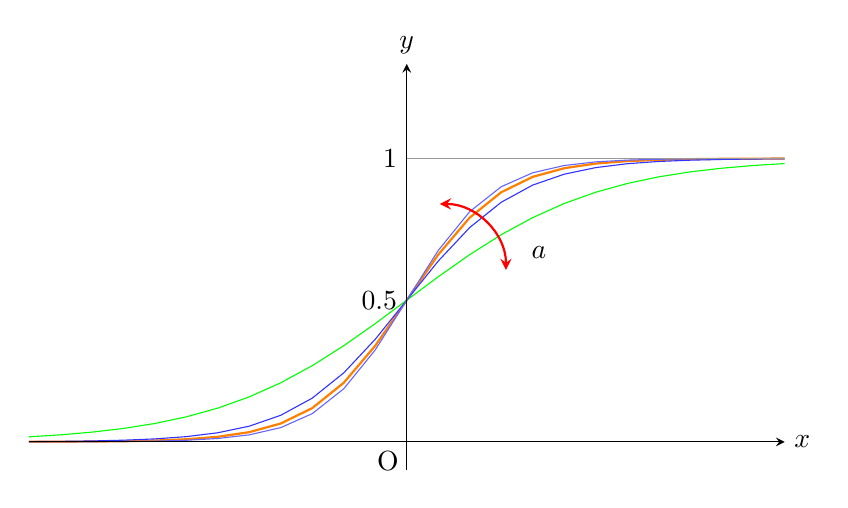
\begin{tikzpicture}[>=stealth,scale=1.2]
        \draw[domain=-4:4,draw=orange,thick] plot(\x,{3/(1+exp(-2*\x))});
        \draw[domain=-4:4,draw=green] plot(\x,{3/(1+exp(-1*\x))});
        \draw[domain=-4:4,draw=blue!80] plot(\x,{3/(1+exp(-1.7*\x))});
        \draw[domain=-4:4,draw=blue!60] plot(\x,{3/(1+exp(-2.2*\x))});
        \draw[draw=gray!80] (4,3)--(0,3) node[left]{$1$};
        \draw(0,1.5)--(0,1.5) node[left] {$0.5$};
        \draw[->](-4,0)--(4,0) node[right]{$x$};
        \draw[->](0,-0.3)--(0,4) node[above]{$y$};
        \node at(-0.2,-0.2) {O};
        \draw[<->,draw=red,thick](60:2.1) arc(0:90:0.7cm);
        \node at(1.4,2) {$a$};
    \end{tikzpicture}
\end{center}
シグモイド関数を$x$軸に$b$だけシフトしたときの関数は以下のように表すことが出来る.
\begin{align*}
    f(x) = \frac{1}{1+{\rm exp}(-a(x-b))}
\end{align*}
すると以下のようにグラフは描くことが可能となる.
\begin{center}
    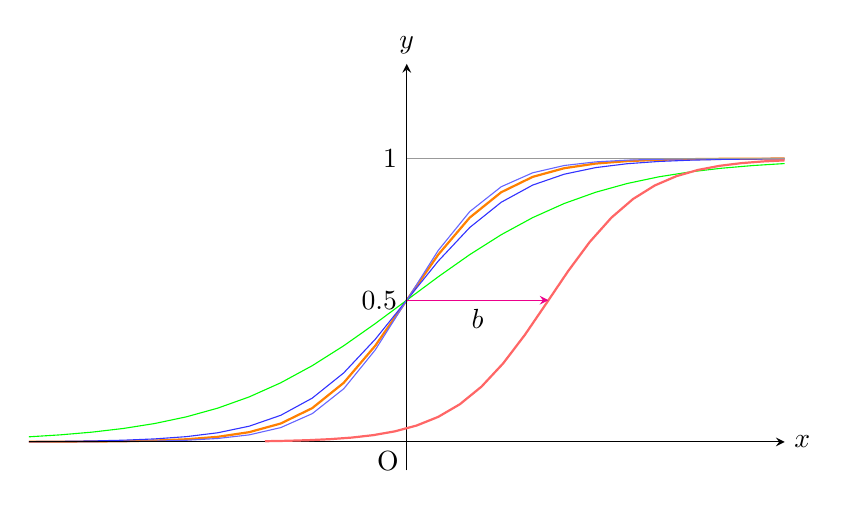
\begin{tikzpicture}[>=stealth,scale=1.2]
        \draw[domain=-4:4,draw=orange,thick] plot(\x,{3/(1+exp(-2*\x))});
        \draw[domain=-4:4,draw=green] plot(\x,{3/(1+exp(-1*\x))});
        \draw[domain=-4:4,draw=blue!80] plot(\x,{3/(1+exp(-1.7*\x))});
        \draw[domain=-4:4,draw=blue!60] plot(\x,{3/(1+exp(-2.2*\x))});
        \draw[draw=gray!80] (4,3)--(0,3) node[left]{$1$};
        \draw(0,1.5)--(0,1.5) node[left] {$0.5$};
        \draw[->](-4,0)--(4,0) node[right]{$x$};
        \draw[->](0,-0.3)--(0,4) node[above]{$y$};
        \node at(-0.2,-0.2) {O};
        \draw[domain=-3:2.5,draw=red!60,thick] plot(\x+1.5,{3/(1+exp(-2*(\x)))});
        \draw[->,draw=magenta](0,1.5)--(1.5,1.5);
        \node at(0.75,1.3) {$b$};
    \end{tikzpicture}
\end{center}
シグモイド関数の重要な性質として微分が元の関数を用いて表現することができる.
\begin{eqnarray*}
    f'(x)&=&\left(\frac{1}{1+{\rm exp}(-x)}\right)'\\
        &=&\frac{{\rm exp}(-x)}{\left(1+{\rm exp}(-x)\right)^{2}}\\
        &=&\frac{1}{1+{\rm exp}(-x)}\cdot \frac{{\rm exp}(-x)}{1+{\rm exp}(-x)}\\
        &=&\frac{1}{1+{\rm exp}(-x)}\cdot \frac{1+{\rm exp}(-x)-1}{1+{\rm exp}(-x)}\\
        &=&\frac{1}{1+{\rm exp}(-x)}\cdot \left(1-\frac{1}{1+{\rm exp}(-x)}\right)\\
        &=&f(x)\left(1-f(x)\right)
\end{eqnarray*}
また, $f'''(x)$については
\begin{eqnarray*}
    f''(x) &=& \left(f'(x)\right)'\\
        &=& \left(f(x)(1-f(x))\right)'\\
        &=& f'(x)(1-f(x))+f(x)(1-f(x))'\\
        &=& f'(x)(1-f(x))-f(x)f'(x)\\
        &=& f'(x)(1-2f(x))\\
        &=& f(x)(1-f(x))(1-2f(x))
\end{eqnarray*}
よって,まとめると
\begin{align*}
    f(x) &= \frac{1}{1+{\rm exp}(-x)}\\
    f'(x)&=f(x)(1-f(x)) \tag {3.3} \\
    f''(x)&=f(x)(1-f(x))(1-2f(x))
\end{align*}
$(x_{n},y_{n})$\ :\ $n$番目の学習データ\\
$\mbox{\boldmath $x$}_{n}=\begin{bmatrix} x_{n}&1 \end{bmatrix}^{T}$\ :\ $x_{n}$を次元拡張してベクトル化したもの\\
$D=\begin{bmatrix}\mbox{\boldmath $x$}_{1}&\mbox{\boldmath $x$}_{2}&\cdots &\mbox{\boldmath $x$}_{n}&\cdots \end{bmatrix}^{T}=\begin{bmatrix}d_{ij}\end{bmatrix},\ (d_{i1}=x_{i},\,d_{i2}=1)$\\
$z_{n}=\mbox{\boldmath $w$}^{T}\mbox{\boldmath $x$}_{n}=\displaystyle \sum_{k}w_{k}\cdot d_{nk}$\\
ここで線形回帰の場合は$\tilde{y}_{n}=f(x_{i};a,b)=ax_{i}+b$としていたが, ロジスティック回帰では\\
$\tilde{y}_{n}=f(z_{n})=\displaystyle \frac{1}{1+{\rm exp}(-z_{n})}$\\[0.1cm]
$\displaystyle E=\frac{1}{2}\sum_{n=1}^{N}(y_{n}-\tilde{y}_{n})^{2}=\frac{1}{2}\sum_{n=1}^{N}\left(y_{n}-\frac{1}{1+{\rm exp}(-z_{n})}\right)^{2}$\\[1cm]
これから誤差$E$が最小となるように計算していくが, ロジスティック回帰の場合は解が解析的に求まらない(微分方程式の解が定まらない)ので, \textcolor{red}{繰り返し計算}が必要となる.\\
ここで, {\bf 勾配法}というものを導入する.
\subsection{勾配法}
勾配法は近似解を与え, 近似解の周辺の傾き等を用いて, 近似解を漸次改良し, この処理をくり返す方法である.\\
(例)\ 最急降下法, 共役勾配法, ニュートン法\\
\begin{center}
    \begin{tikzpicture}[>=stealth]
        \draw[fill=gray!20,rotate=50,xscale=1.9] (1.5,2) circle[radius=2];
        \draw[fill=gray!30,rotate=50,xscale=1.9] (1.7,2) circle[radius=1.7];
        \draw[fill=gray!40,rotate=50,xscale=1.9] (1.8,2) circle[radius=1.5];
        \draw[fill=gray!60,rotate=50,xscale=2] (1.8,2) circle[radius=1.3];
        \draw[fill=gray!70,rotate=51,xscale=2] (2,1.9) circle[radius=1];
        \draw[fill=magenta,draw=black] (-2,2) circle[radius=0.1];
        \draw(-2.1,2)--(-2.1,2) node[left]{$\mbox{\boldmath $x$}_{0}$};
        \draw[->,draw=green,very thick] (-1.9,2)--(-1.1,2);
        \node at(-1.5,1.7) {$-\nabla f(\mbox{\boldmath $x$}_{0})$};
        \node at(-1.5,1.35) {$H(\mbox{\boldmath $x$}_{0})$};
        \draw[->,draw=blue] (-1.9,2.05)--(-0.6,2.45);
        \draw[fill=magenta,draw=black] (-0.5,2.5) circle[radius=0.1];
        \draw(-0.5,2.4)--(-0.5,2.4) node[below] {$\mbox{\boldmath $x$}_{1}$};
        \draw[->,draw=green,very thick] (-0.42,2.55)--(0.32,3.55);
        \draw[->,draw=blue] (-0.42,2.55)--(1.03,3.93);
        \node at(0.8,3) {$-\nabla f(\mbox{\boldmath $x$}_{1})$};
        \node at(0.8,2.65) {$H(\mbox{\boldmath $x$}_{1})$};
        \draw[fill=magenta,draw=black] (1.1,4) circle[radius=0.1];
        \draw (1.1,4.05)--(1.1,4.05) node[above left] {$\mbox{\boldmath $x$}_{2}$};
        \draw[->,draw=green,very thick] (1.15,4.1)--(1.49,4.86);
        \draw[->,draw=blue] (1.15,4.1)--(1.84,5.17);
        \node at(2.2,4.6) {$-\nabla f(\mbox{\boldmath $x$}_{2})$};
        \node at(2.2,4.25) {$H(\mbox{\boldmath $x$}_{2})$};
        \draw[fill=red] (1.9,5.3) circle[radius=0.15];
        \node at(-2.3,3) {適当な初期値};
    \end{tikzpicture}
\end{center}
このように近似解を繰り返し修正することで最適値へ近づいていく. 勾配(, ヘシアン), つまり$E$の$\mbox{\boldmath $x$}_{0}$における1次(,2次)の微分)施すことで修正を行う. \\
問題としては近似解の精度を上げるために\textcolor{red}{どちらの方向にどれだけ}動かすか?ということである.
\subsubsection{最急降下法}
最急降下法は最も単純なもので勾配の方向に適当量移動させるという方法である. 式にすると以下のように表すことができる.
\begin{align*}
    x_{i+1}=x_{i}-\alpha \nabla f(\mbox{\boldmath $x$}_{i}) \tag{3.4}
\end{align*}
イメージ図としては以下のようになる.
\begin{center}
    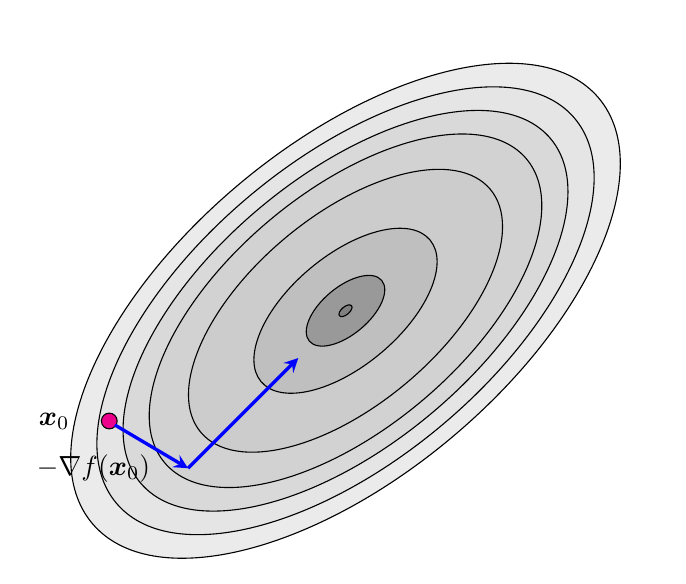
\begin{tikzpicture}[>=stealth]
        \draw[rotate=40,fill=gray!16,xscale=2] circle[radius=2.1];
        \draw[rotate=40,fill=gray!20,xscale=2] circle[radius=1.9];
        \draw[rotate=40,fill=gray!30,xscale=2] circle[radius=1.7];
        \draw[rotate=40,fill=gray!35,xscale=2] circle[radius=1.5];
        \draw[rotate=40,fill=gray!40,xscale=2] circle[radius=1.2];
        \draw[rotate=40,fill=gray!50,xscale=2] circle[radius=0.7];
        \draw[rotate=40,fill=gray!80,xscale=2] circle[radius=0.3];
        \draw[rotate=40,fill=gray,xscale=2] circle[radius=0.05];
        \draw[fill=magenta] (-3,-1.4) circle[radius=0.1];
        \draw[->,very thick,draw=blue] (-2.93,-1.45)--(-2,-2);
        \draw[->,very thick,draw=blue] (-2,-2)--(-0.6,-0.6);
        \node at(-3.2,-2) {$-\nabla f(\mbox{\boldmath $x$}_{0})$};
        \node at(-3.7,-1.4) {$\mbox{\boldmath $x$}_{0}$};
    \end{tikzpicture}
\end{center}
誤差が最小となるところに持っていく. ということは誤差関数において値が最小となるように持ってくることである. つまり誤差関数の現時点にいる場所から傾きを得る. それが負であれば$+$にずらし, 正なら$-$にずらすことで最小値に近づけることが可能となる. 誤差関数が二次関数においての例は以下である.
\begin{center}
    \begin{tikzpicture}[>=stealth]
    \draw[very thick,domain=-3:3] plot(\x,{\x*\x/2});
    \draw[->] (-3,0)--(3,0) node[right] {$x$};
    \draw[->] (0,-0.3)--(0,5) node[above] {$y$};
    \node at(-0.2,-0.2) {O};
    \draw[thick,domain=1.5:2.5,draw=red] plot(\x,{2*\x-2});
    \draw[fill=magenta] (2,2) circle[radius=0.08];
    \draw[fill=magenta] (-2,2) circle[radius=0.08];
    \node at(4.3,2) {傾きが$+$なので$-$方向へ};
    \draw[thick,domain=-2.5:-1.5,draw=red] plot(\x,{-2*\x-2});
    \node at(-4.3,2) {傾きが$-$なので$+$方向へ};
    \end{tikzpicture}
\end{center}
最急降下法のアルゴリズムは以下のように表すことができる.\\[0.1cm]
$i_{0},\ x_{0}$を決める.\\
収束するまで繰り返し\{\\
\hspace{1cm} $x_{i+1}=x_{i}-\alpha \nabla f(\mbox{\boldmath $x$}_{i})$\\
\hspace{1cm} $i=i+1$\\
\}\\[0.1cm]
$\alpha$の決め方は様々であり, $-\nabla f(\mbox{\boldmath $x$})$の最適値を解析的に求めるかラインサーチによって求めて移動する. このときの移動量は同じであるが過去の勾配の大きさの履歴に応じて移動量を決定する.
\begin{center}
    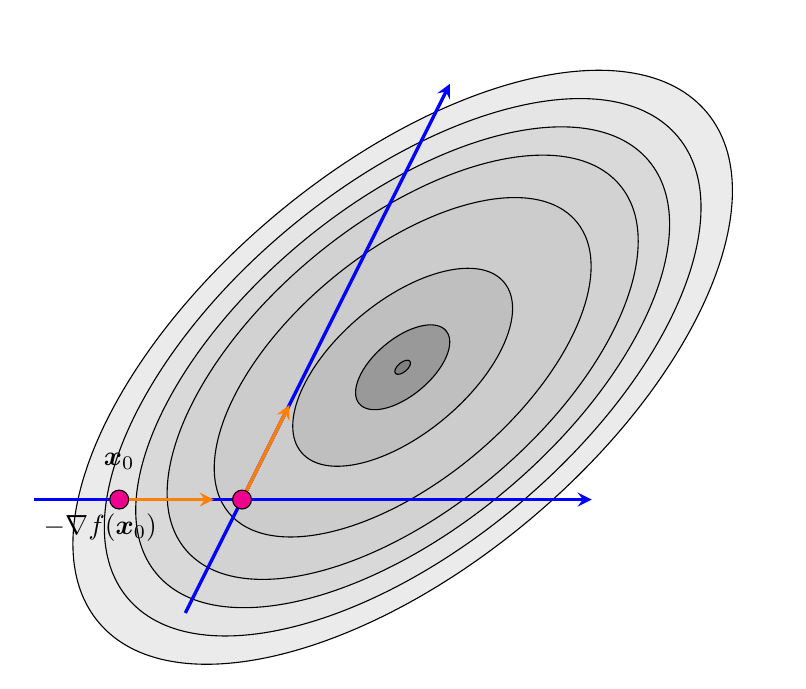
\begin{tikzpicture}[scale=1.2,>=stealth]
        \draw[rotate=40,fill=gray!16,xscale=2] circle[radius=2.1];
        \draw[rotate=40,fill=gray!20,xscale=2] circle[radius=1.9];
        \draw[rotate=40,fill=gray!30,xscale=2] circle[radius=1.7];
        \draw[rotate=40,fill=gray!35,xscale=2] circle[radius=1.5];
        \draw[rotate=40,fill=gray!40,xscale=2] circle[radius=1.2];
        \draw[rotate=40,fill=gray!50,xscale=2] circle[radius=0.7];
        \draw[rotate=40,fill=gray!80,xscale=2] circle[radius=0.3];
        \draw[rotate=40,fill=gray,xscale=2] circle[radius=0.05];
        \draw[->,very thick,draw=blue] (-3.9,-1.4)--(2,-1.4);
        \draw[->,very thick,draw=blue] (-2.3,-2.6)--(0.5,3);

        \draw[->,very thick,draw=orange](-1.7,-1.4)--(-1.2,-0.4); 
        \draw[fill=magenta] (-3,-1.4) circle[radius=0.1];
        \draw[fill=magenta] (-1.7,-1.4) circle[radius=0.1];
        \node at(-3.2,-1.7) {$-\nabla f(\mbox{\boldmath $x$}_{0})$};
        \node at(-3,-1) {$\mbox{\boldmath $x$}_{0}$};
        \draw[->,very thick,draw=orange](-2.9,-1.4)--(-2,-1.4);
    \end{tikzpicture}
\end{center}
以下の関数の最小値を最急降下法で求めてみる.
\begin{eqnarray*}
    f(\mbox{\boldmath $x$}) = \frac{1}{2}\mbox{\boldmath $x$}^{T}\begin{pmatrix}6&1\\1&2\end{pmatrix}\mbox{\boldmath $x$}-\begin{pmatrix}2\\1\end{pmatrix}^{T}\mbox{\boldmath $x$}
\end{eqnarray*}
これの初期値として$\mbox{\boldmath $x$}=\begin{pmatrix}0\\0\end{pmatrix}$としてpythonで実装した場合は以下のようになる.
\lstinputlisting{grad.py}

実行結果として, 最小値は$\begin{pmatrix}0.27281847\\0.36325003\end{pmatrix}$が得られる.\\
$\alpha$の値を移動量を最初大きくし, 最適解に近づくにつれてだんだん小さくした場合のpythonの実装は以下のようになる.
\lstinputlisting{grad2.py}
実行結果として, 最小値は$\begin{pmatrix}0.27279382\\0.36320777\end{pmatrix}$が得られる.\\[1cm]
関数$\displaystyle f(x)=\frac{1}{2}\mbox{\boldmath $x$}^{T}A\mbox{\boldmath $x$}-\mbox{\boldmath $b$}^{T}\mbox{\boldmath $x$}$の最小値を与える$\alpha$について解析的に求める方法はまず変数$\mbox{\boldmath $x$}$について
\begin{eqnarray*}
    \mbox{\boldmath $x$} = \mbox{\boldmath $x$}_{0}+\alpha \mbox{\boldmath $d$}
\end{eqnarray*}
とおき, これを代入することで計算していく.
まず
\begin{eqnarray*}
    f(x) &=& f(\mbox{\boldmath $x$}_{0}+\alpha\mbox{\boldmath $d$})\\
    f(\alpha) &=& \frac{1}{2}(\mbox{\boldmath $x$}_{0}+\alpha \mbox{\boldmath $d$})^{T}A(\mbox{\boldmath $x$}_{0}+\alpha \mbox{\boldmath $d$})-\mbox{\boldmath $b$}^{T}(\mbox{\boldmath $x$}_{0}+\alpha \mbox{\boldmath $d$})
\end{eqnarray*}
最小値を与える$\alpha$であるので極値を求めればよく,
\begin{eqnarray*}
    \frac{d}{d\alpha}f(\alpha) = 0
\end{eqnarray*}
が成立すればよい.
したがってこれを計算すると
\begin{eqnarray*}
    &&\frac{d}{d\alpha}f(\alpha) = 0\\
    \Longleftrightarrow \ && (\mbox{\boldmath $x$}_{0}+\alpha \mbox{\boldmath $d$})^{T}A\mbox{\boldmath $d$}-\mbox{\boldmath $b$}^{T}\mbox{\boldmath $d$} = 0\\
    \Longleftrightarrow\ && \alpha \mbox{\boldmath $d$}^{T}A\mbox{\boldmath $d$}+\mbox{\boldmath $x$}_{0}^{T}A\mbox{\boldmath $d$}-\mbox{\boldmath $b$}^{T}\mbox{\boldmath $d$} = 0\\
    \Longleftrightarrow \ && \alpha \mbox{\boldmath $d$}^{T}A\mbox{\boldmath $d$}+\nabla f(\mbox{\boldmath $x$}_{0})^{T}\mbox{\boldmath $d$}=0\\
    \Longleftrightarrow\ && \alpha = -\frac{\nabla f(\mbox{\boldmath $x$}_{0})^{T}\mbox{\boldmath $d$}}{\mbox{\boldmath $d$}^{T}A\mbox{\boldmath $d$}}
\end{eqnarray*}
\subsubsection{共役勾配法}
最急降下法では, 直線的に最適解に向かわないので今まで進んできた方向と共役な方向に移動方向を決める方法を共役勾配法という.
\begin{center}
    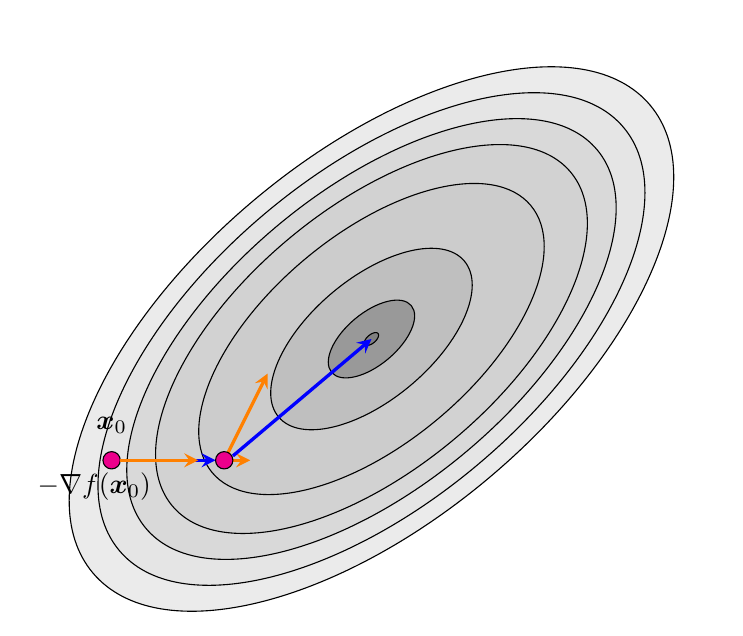
\begin{tikzpicture}[scale=1.1,>=stealth]
        \draw[rotate=40,fill=gray!16,xscale=2] circle[radius=2.1];
        \draw[rotate=40,fill=gray!20,xscale=2] circle[radius=1.9];
        \draw[rotate=40,fill=gray!30,xscale=2] circle[radius=1.7];
        \draw[rotate=40,fill=gray!35,xscale=2] circle[radius=1.5];
        \draw[rotate=40,fill=gray!40,xscale=2] circle[radius=1.2];
        \draw[rotate=40,fill=gray!50,xscale=2] circle[radius=0.7];
        \draw[rotate=40,fill=gray!80,xscale=2] circle[radius=0.3];
        \draw[rotate=40,fill=gray,xscale=2] circle[radius=0.05];
        \draw[->,very thick,draw=blue] (-2.9,-1.4)--(-1.8,-1.4);

        \draw[->,very thick,draw=orange](-1.7,-1.4)--(-1.2,-0.4);
        \draw[->,very thick,draw=orange](-1.6,-1.4)--(-1.4,-1.4);
        \draw[->,very thick,draw=blue] (-1.6,-1.35)--(0,0);
        \draw[fill=magenta] (-3,-1.4) circle[radius=0.1];
        \draw[fill=magenta] (-1.7,-1.4) circle[radius=0.1];
        \node at(-3.2,-1.7) {$-\nabla f(\mbox{\boldmath $x$}_{0})$};
        \node at(-3,-1) {$\mbox{\boldmath $x$}_{0}$};
        \draw[->,very thick,draw=orange](-2.9,-1.4)--(-2,-1.4);
    \end{tikzpicture}
\end{center}
共役勾配法を式にすると以下のように表すことができる.
\begin{align*}
    \begin{array}{l}
    \mbox{\boldmath $x$}_{k}=\mbox{\boldmath $x$}_{k-1}+c_{k}\mbox{\boldmath $p$}_{k}\\
    \mbox{\boldmath $p$}_{k+1}=-\nabla f(\mbox{\boldmath $x$}_{k})+\alpha_{k}\mbox{\boldmath $p$}_{k}
    \end{array} \tag{3.5}
\end{align*}
共役勾配法は勾配だけでなく, \textcolor{red}{今まで進んできた方向も考慮して}探索の方向を決めることで効率化を図っている. 「今までの進んできた方向の考慮」にあたり, \textcolor{red}{ベクトルの共役}という性質を利用する.\\
共役とは, $\mbox{\boldmath $x$},\ \mbox{\boldmath $y$}$が,
\begin{eqnarray*}
    \mbox{\boldmath $x$}^{T}A\mbox{\boldmath $y$}=\langle \mbox{\boldmath $x$},\mbox{\boldmath $y$}\rangle_{A}=0
\end{eqnarray*}
を満たすことをいう.\\
固有ベクトルによる対称行列の対角化を行う.\ $n$次対称行列$A$は\\
固有ベクトル$\mbox{\boldmath $v$}_{1},\mbox{\boldmath $v$}_{2},\cdots,\mbox{\boldmath $v$}_{n}$を並べて作る行列
\begin{eqnarray*}
    V=\begin{pmatrix}\mbox{\boldmath $v$}_{1}&\mbox{\boldmath $v$}_{2}&\cdots&\mbox{\boldmath $v$}_{n}\end{pmatrix}
\end{eqnarray*}
を用いて
\begin{eqnarray*}
    V^{T}AV &=& \Lambda\\
    \Lambda&=&\begin{pmatrix}\lambda_{1}&&&0\\ & \lambda_{2}&&\\ &&\ddots& \\ 0&&&\lambda_{n}\end{pmatrix}
\end{eqnarray*}
ここで, $\lambda_{1},\lambda_{2},\cdots,\lambda_{n}$は固有値であり, このように対角化することが可能となる.\\
ここで$V^{T}V=VV^{T}=I$であるから
\begin{eqnarray*}
    VV^{T}AVV^{T}=V\Lambda V^{T},\ \ A=V\Lambda V^{T}
\end{eqnarray*}
となる. したがって, 対称行列は固有値を対角要素に持つ行列$\Lambda$と固有ベクトルをならべて作る行列$V$で表すことができる\\
したがって共役な$\mbox{\boldmath $x$}_{1},\mbox{\boldmath $x$}_{2}$ついて
\begin{eqnarray*}
    \mbox{\boldmath $x$}_{1}^{T}A\mbox{\boldmath $x$}_{2}&=&\mbox{\boldmath $x$}_{1}^{T}V\Lambda V^{T}\mbox{\boldmath $x$}_{2}\\
                                                        &=&\mbox{\boldmath $x$}_{1}^{T}V\Lambda^{\frac{1}{2}}\Lambda^{\frac{1}{2}}V^{T}\mbox{\boldmath $x$}_{2}\\
                                                        &=&\mbox{\boldmath $x$}_{1}^{T}V\Lambda^{\frac{1}{2}T}\Lambda^{\frac{1}{2}}V^{T}\mbox{\boldmath $x$}_{2}\\
                                                        &=&\mbox{\boldmath $x$}_{1}^{T}\left(\Lambda^{\frac{1}{2}}V^{T}\right)^{T}\Lambda^{\frac{1}{2}}V^{T}\mbox{\boldmath $x$}_{2}\\
    &=&\left(\Lambda^{\frac{1}{2}}V^{T}\mbox{\boldmath $x$}_{1}\right)^{T}\Lambda^{\frac{1}{2}}V^{T}\mbox{\boldmath $x$}_{2}
\end{eqnarray*}
$\Lambda$は対角行列であるのでその平方根である$\Lambda^{\frac{1}{2}}$も対角行列となる. また対角行列の転置行列は元の行列と等しいことを考慮して先のように変形することが出来る.\ ここでベクトル$z$に対して
\begin{eqnarray*}
    \mbox{\boldmath $z$}=\Lambda^{\frac{1}{2}}V^{T}\mbox{\boldmath $x$}
\end{eqnarray*}
なる座標変換をした後のベクトルについて考える.\\
\begin{eqnarray*}
    \mbox{\boldmath $z$}&=&\Lambda^{\frac{1}{2}}V^{T}\mbox{\boldmath $x$}\\
    \mbox{\boldmath $z$}&=&\Lambda^{\frac{1}{2}}\mbox{\boldmath $y$}\\
    \mbox{\boldmath $y$}&=&V^{T}\mbox{\boldmath $x$}
\end{eqnarray*}
とする. そして以下の平面について考える.
\begin{center}
    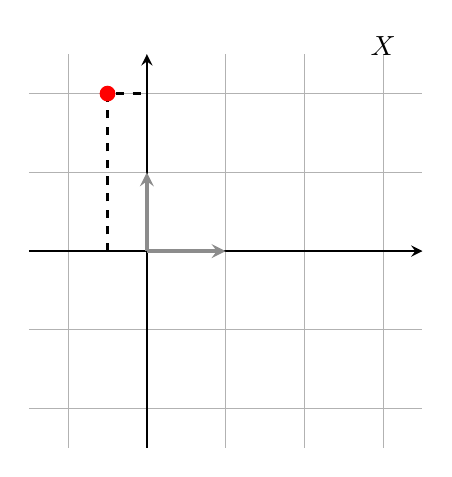
\begin{tikzpicture}[>=stealth]
        \draw[draw=gray!60](-1.5,-2.5) grid (3.5,2.5);
        \draw[thick,->](-1.5,0)--(3.5,0);
        \draw[thick,->](0,-2.5)--(0,2.5);
        \draw[very thick,draw=gray!90,->] (0,0)--(0,1);
        \draw[very thick,draw=gray!90,->] (0,0)--(1,0);
        \draw[dashed,thick](-0.5,0)--(-0.5,2)--(0,2);
        \fill[fill=red] (-0.5,2) circle[radius=0.1];
        \node at(3,2.6) {$X$};
    \end{tikzpicture}
\end{center}
これから$\mbox{\boldmath $y$}$について変換を行うと
\begin{eqnarray*}
    \begin{pmatrix}y_{1}\\y_{2}\end{pmatrix}=\begin{pmatrix}\mbox{\boldmath $v$}_{1}^{T}\mbox{\boldmath $x$}\\\mbox{\boldmath $v$}_{2}^{T}\mbox{\boldmath $x$}\end{pmatrix}
\end{eqnarray*}
となるので$Y$についての平面は以下のように表すことができる.
\begin{center}
    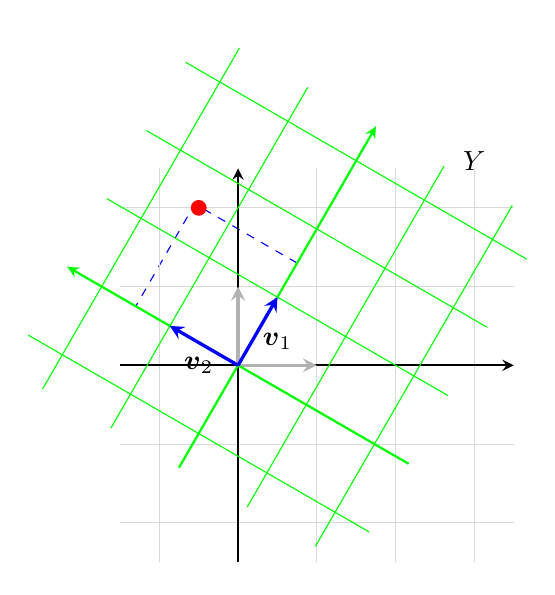
\begin{tikzpicture}[>=stealth]
        \draw[dashed,draw=blue,rotate=60] (1.5,0)--(1.5,1.5)--(0,1.5);
        \draw[draw=gray!30](-1.5,-2.5) grid (3.5,2.5);
        \draw[thick,->](-1.5,0)--(3.5,0);
        \draw[thick,->](0,-2.5)--(0,2.5);
        \draw[very thick,draw=gray!60,->] (0,0)--(0,1);
        \draw[very thick,draw=gray!60,->] (0,0)--(1,0);
        \fill[fill=red] (-0.5,2) circle[radius=0.1];
        \draw[draw=green,rotate=60](-1.5,-2.5) grid (3.5,2.5);
        \draw[thick,->,draw=green,rotate=60](-1.5,0)--(3.5,0);
        \draw[thick,->,draw=green,rotate=60](0,-2.5)--(0,2.5);
        \draw[very thick,draw=blue,->,rotate=60] (0,0)--(0,1);
        \draw[very thick,draw=blue,->,rotate=60] (0,0)--(1,0);

        \node at(3,2.6) {$Y$};
        \node at(0.5,0.3) {$\mbox{\boldmath $v$}_{1}$};
        \node at(-0.5,0) {$\mbox{\boldmath $v$}_{2}$};
    \end{tikzpicture}
\end{center}
これに加えて$\mbox{\boldmath $z$}$に関して,
\begin{eqnarray*}
    \begin{pmatrix}z_{1}\\z_{2}\end{pmatrix}=\begin{pmatrix}\sqrt{\mbox{\boldmath $\lambda$}_{1}}y_{1}\\\sqrt{\mbox{\boldmath $\lambda$}_{1}}y_{1}\end{pmatrix} 
\end{eqnarray*}
となるので固有値の平方根をとることで$Z$についての平面は以下のようになる.
\begin{center}
    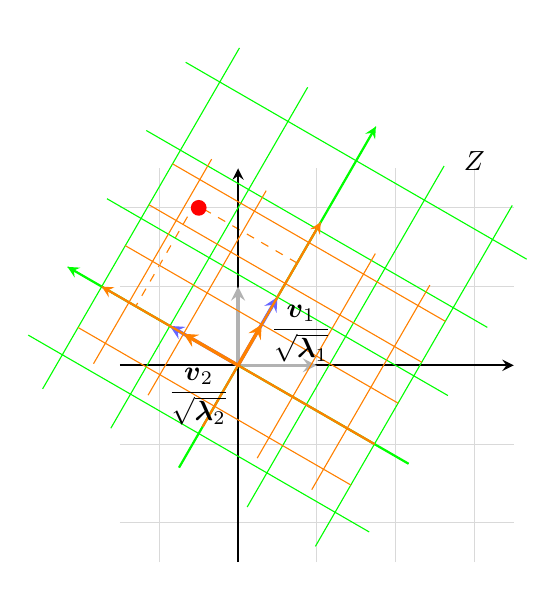
\begin{tikzpicture}[>=stealth]
        \draw[dashed,draw=orange,rotate=60] (1.5,0)--(1.5,1.5)--(0,1.5);
        \draw[draw=gray!30](-1.5,-2.5) grid (3.5,2.5);
        \draw[thick,->](-1.5,0)--(3.5,0);
        \draw[thick,->](0,-2.5)--(0,2.5);
        \draw[very thick,draw=gray!60,->] (0,0)--(0,1);
        \draw[very thick,draw=gray!60,->] (0,0)--(1,0);
        \fill[fill=red] (-0.5,2) circle[radius=0.1];
        \draw[draw=green,rotate=60](-1.5,-2.5) grid (3.5,2.5);
        \draw[thick,->,draw=green,rotate=60](-1.5,0)--(3.5,0);
        \draw[thick,->,draw=green,rotate=60](0,-2.5)--(0,2.5);
        \draw[very thick,draw=blue!60,->,rotate=60] (0,0)--(0,1);
        \draw[very thick,draw=blue!60,->,rotate=60] (0,0)--(1,0);
        \draw[draw=orange,rotate=60,xscale=0.6,yscale=0.8](-1.5,-2.5) grid (3.5,2.5);
        \draw[thick,->,draw=orange,rotate=60,xscale=0.6,yscale=0.8](-1.5,0)--(3.5,0);
        \draw[thick,->,draw=orange,rotate=60,xscale=0.6,yscale=0.8](0,-2.5)--(0,2.5);
        \draw[very thick,draw=orange,->,rotate=60,xscale=0.6,yscale=0.8] (0,0)--(0,1);
        \draw[very thick,draw=orange,->,rotate=60,xscale=0.6,yscale=0.8] (0,0)--(1,0);

        \node at(3,2.6) {$Z$};
        \node at(0.8,0.4) {$\displaystyle \frac{\mbox{\boldmath $v$}_{1}}{\sqrt{\mbox{\boldmath $\lambda$}_{1}}}$};
        \node at(-0.5,-0.4) {$\displaystyle \frac{\mbox{\boldmath $v$}_{2}}{\sqrt{\mbox{\boldmath $\lambda$}_{2}}}$};
    \end{tikzpicture}
\end{center}
座標変換後の直交とは
\begin{eqnarray*}
    \mbox{\boldmath $z$}_{a}^{T}\cdot \mbox{\boldmath $z$}_{b}=0
\end{eqnarray*}
が成立することである.
\begin{center}
    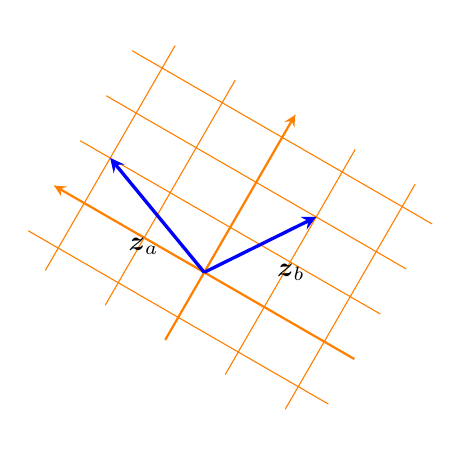
\begin{tikzpicture}[>=stealth,scale=1.1]
        \draw[draw=orange,rotate=60,xscale=0.6,yscale=0.8](-1.5,-2.5) grid (3.5,2.5);
        \draw[thick,->,draw=orange,rotate=60,xscale=0.6,yscale=0.8](-1.5,0)--(3.5,0);
        \draw[thick,->,draw=orange,rotate=60,xscale=0.6,yscale=0.8](0,-2.5)--(0,2.5);
        \draw[rotate=60,very thick,draw=blue,->,xscale=0.6,yscale=0.8] (0,0)--(1,2);
        \draw[rotate=60,very thick,draw=blue,->,xscale=0.6,yscale=0.8] (0,0)--(2,-1);
        \node at(-0.7,0.3) {$\mbox{\boldmath $z$}_{a}$};
        \node at(1,0) {$\mbox{\boldmath $z$}_{b}$};
    \end{tikzpicture}
\end{center}
これについて元の座標においては共役である. つまり
\begin{eqnarray*}
    \mbox{\boldmath $x$}_{a}^{T}A\mbox{\boldmath $x$}_{b}=0
\end{eqnarray*}
ということである.
\begin{center}
    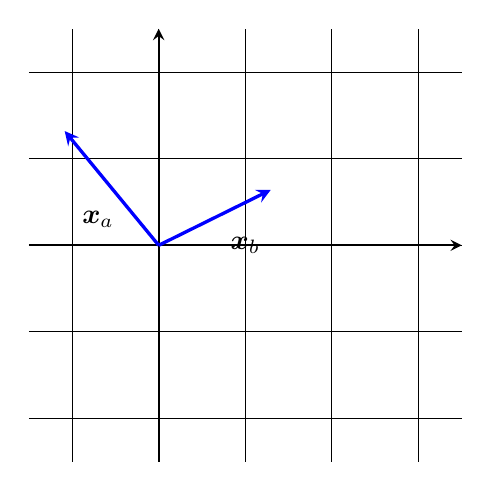
\begin{tikzpicture}[>=stealth,scale=1.1]
        \draw(-1.5,-2.5) grid (3.5,2.5);
        \draw[thick,->](-1.5,0)--(3.5,0);
        \draw[thick,->](0,-2.5)--(0,2.5);
        \draw[rotate=60,very thick,draw=blue,->,xscale=0.6,yscale=0.8] (0,0)--(1,2);
        \draw[rotate=60,very thick,draw=blue,->,xscale=0.6,yscale=0.8] (0,0)--(2,-1);
        \node at(-0.7,0.3) {$\mbox{\boldmath $x$}_{a}$};
        \node at(1,0) {$\mbox{\boldmath $x$}_{b}$};
    \end{tikzpicture}
\end{center}                       
円については座標変換後の円が
\begin{eqnarray*}
    \mbox{\boldmath $z$}^{T}\cdot \mbox{\boldmath $z$} = {\rm const}
\end{eqnarray*}
とする.
\begin{center}
    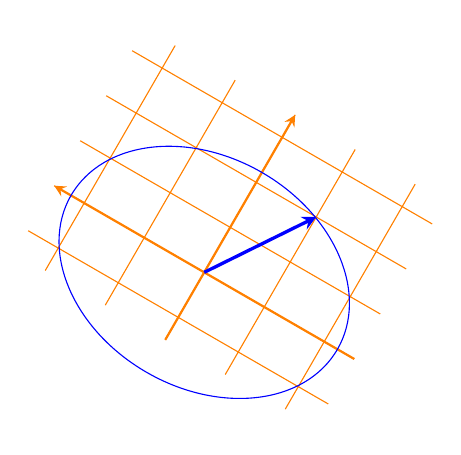
\begin{tikzpicture}[>=stealth,scale=1.1]
        \draw[draw=orange,rotate=60,xscale=0.6,yscale=0.8](-1.5,-2.5) grid (3.5,2.5);
        \draw[thick,->,draw=orange,rotate=60,xscale=0.6,yscale=0.8](-1.5,0)--(3.5,0);
        \draw[thick,->,draw=orange,rotate=60,xscale=0.6,yscale=0.8](0,-2.5)--(0,2.5);
        \draw[rotate=60,very thick,draw=blue,->,xscale=0.6,yscale=0.8] (0,0)--(2,-1);
        \draw[rotate=60,draw=blue,xscale=0.6,yscale=0.8] (0,0) circle[yscale=1.85,xscale=1.85,radius=1.2];
    \end{tikzpicture}
\end{center}
これを元の座標では楕円であり以下の式を満たす
\begin{eqnarray*}
    \mbox{\boldmath $x$}^{T}A\mbox{\boldmath $x$} = {\rm const}
\end{eqnarray*}
このとき半径(長半径, 短半径)は, 固有値の平方根の逆数となる.
\begin{center}
    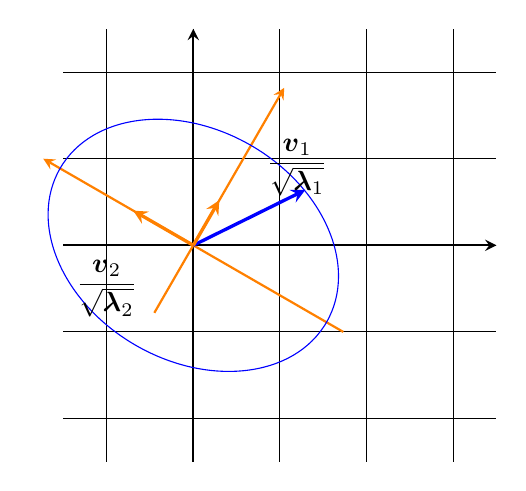
\begin{tikzpicture}[>=stealth,scale=1.1]
        \draw(-1.5,-2.5) grid (3.5,2.5);
        \draw[thick,->](-1.5,0)--(3.5,0);
        \draw[thick,->](0,-2.5)--(0,2.5);
        \draw[thick,->,draw=orange,rotate=60,xscale=0.6,yscale=0.8](-1.5,0)--(3.5,0);
        \draw[thick,->,draw=orange,rotate=60,xscale=0.6,yscale=0.8](0,-2.5)--(0,2.5);
        \draw[rotate=60,very thick,draw=blue,->,xscale=0.6,yscale=0.8] (0,0)--(2,-1);
        \draw[rotate=60,draw=blue,xscale=0.6,yscale=0.8] (0,0) circle[yscale=1.85,xscale=1.85,radius=1.2];
        \draw[rotate=60,draw=orange,very thick,->,xscale=0.6,yscale=0.8] (0,0)--(1,0);
        \draw[rotate=60,draw=orange,very thick,->,xscale=0.6,yscale=0.8] (0,0)--(0,1);
        \node at(1.2,0.9) {$\displaystyle \frac{\mbox{\boldmath $v$}_{1}}{\sqrt{\mbox{\boldmath $\lambda$}_{1}}}$};
        \node at(-1,-0.5) {$\displaystyle \frac{\mbox{\boldmath $v$}_{2}}{\sqrt{\mbox{\boldmath $\lambda$}_{2}}}$};
    \end{tikzpicture}
\end{center}
つまり共役の方向に近似解を更新するということは, 楕円を円に変換したときに直行する方向に近似解を更新することに相当する.
\begin{center}
    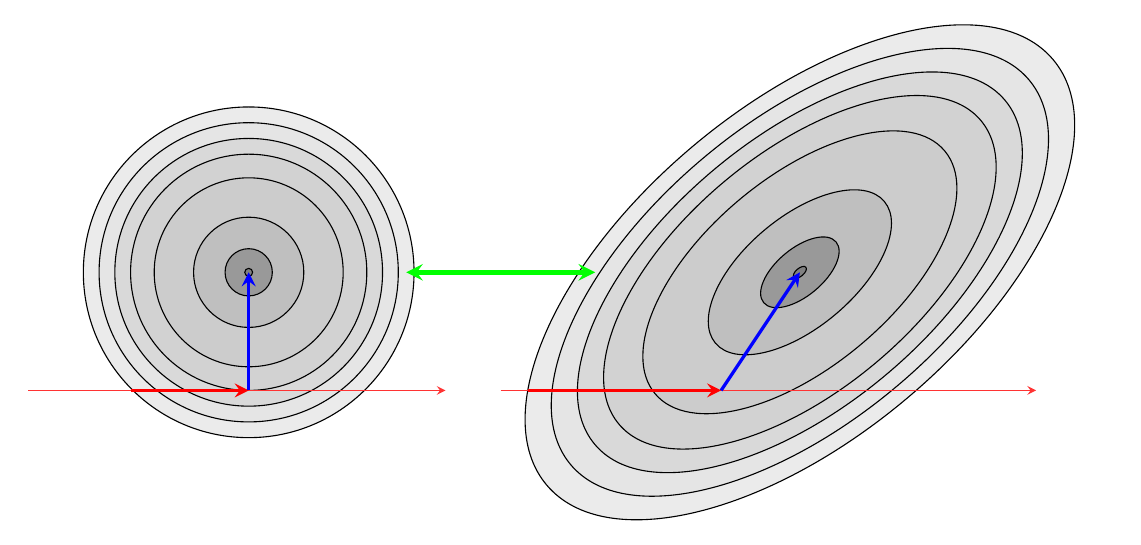
\begin{tikzpicture}[>=stealth]
        \draw[rotate=40,fill=gray!16,xscale=2] (0,0) circle[radius=2.1];
        \draw[rotate=40,fill=gray!20,xscale=2] (0,0) circle[radius=1.9];
        \draw[rotate=40,fill=gray!30,xscale=2] (0,0) circle[radius=1.7];
        \draw[rotate=40,fill=gray!35,xscale=2] (0,0) circle[radius=1.5];
        \draw[rotate=40,fill=gray!40,xscale=2] (0,0) circle[radius=1.2];
        \draw[rotate=40,fill=gray!50,xscale=2] (0,0) circle[radius=0.7];
        \draw[rotate=40,fill=gray!80,xscale=2] (0,0) circle[radius=0.3];
        \draw[rotate=40,fill=gray,xscale=2] (0,0) circle[radius=0.05];

        \draw[fill=gray!16] (-7,0) circle[radius=2.1];
        \draw[fill=gray!20] (-7,0) circle[radius=1.9];
        \draw[fill=gray!30] (-7,0) circle[radius=1.7];
        \draw[fill=gray!35] (-7,0) circle[radius=1.5];
        \draw[fill=gray!40] (-7,0) circle[radius=1.2];
        \draw[fill=gray!50] (-7,0) circle[radius=0.7];
        \draw[fill=gray!80] (-7,0) circle[radius=0.3];
        \draw[fill=gray] (-7,0) circle[radius=0.05];
        \draw[draw=red!80,->] (-9.8,-1.5)--(-4.5,-1.5);
        \draw[draw=red,very thick,->] (-8.5,-1.5)--(-7,-1.5);
        \draw[draw=blue,very thick,->] (-7,-1.5)--(-7,0);
        \draw[draw=red!80,->] (-3.8,-1.5)--(3,-1.5);
        \draw[draw=red,->,very thick] (-3.45,-1.5)--(-1,-1.5);
        \draw[draw=blue,->,very thick] (-1,-1.5)--(0,0);
        \draw[<->,ultra thick,draw=green] (-5,0)--(-2.6,0);
    \end{tikzpicture}
\end{center}
$A$を$N$次正定値対称行列として, 互いな共役なベクトル$\mbox{\boldmath $p$}_{1},\mbox{\boldmath $p$}_{2},\mbox{\boldmath $p$}_{3},\cdots ,\mbox{\boldmath $p$}_{N}$を用いて,
\begin{eqnarray*}
    A\mbox{\boldmath $x$} = \mbox{\boldmath $b$}
\end{eqnarray*}
の解$\mbox{\boldmath $x$}^{*}$を表現することを考える.
\begin{eqnarray*}
    \mbox{\boldmath $x$}^{*}=\sum_{k=1}^{N}c_{k}\mbox{\boldmath $p$}_{k}
\end{eqnarray*}
とおくと, \\
$\mbox{\boldmath $p$}_{i}$は, $\mbox{\boldmath $p$}_{j}\ (j\neq i)$は共役であるから,
\begin{eqnarray*}
    &&\mbox{\boldmath $p$}_{i}^{T}A\mbox{\boldmath $x$}^{*}=\mbox{\boldmath $p$}_{i}^{T}\sum_{k=1}^{N}c_{k}A\mbox{\boldmath $p$}_{k}=c_{i}\mbox{\boldmath $p$}_{i}^{T}A\mbox{\boldmath $p$}_{i}=\mbox{\boldmath $p$}_{i}^{T}\mbox{\boldmath $b$}\\
    \Longrightarrow&&\ c_{i}=\frac{\mbox{\boldmath $p$}_{i}^{T}\mbox{\boldmath $b$}}{\mbox{\boldmath $p$}_{i}^{T}A\mbox{\boldmath $p$}_{i}}
\end{eqnarray*}
として$c_{i}$を定めることができる.\\[0.5cm]
共役勾配法の2次形式の場合の解を求めてみる. つまり
\begin{eqnarray*}
    f(\mbox{\boldmath $x$})=\frac{1}{2}\mbox{\boldmath $x$}^{T}A\mbox{\boldmath $x$}-\mbox{\boldmath $b$}^{T}\mbox{\boldmath $x$}
\end{eqnarray*}
に対して
\begin{eqnarray*}
    \nabla f(\mbox{\boldmath $x$})=A\mbox{\boldmath $x$}-\mbox{\boldmath $b$}=0
\end{eqnarray*}
すなわち
\begin{eqnarray*}
    A\mbox{\boldmath $x$}=\mbox{\boldmath $b$}
\end{eqnarray*}
の解を求める.\\
適当な初期値$\mbox{\boldmath $x$}_{0}$を定め, その負の勾配を$\mbox{\boldmath $r$}_{0}$とする.
\begin{eqnarray*}
    \mbox{\boldmath $r$}_{0}=-\nabla f(\mbox{\boldmath $x$}_{0}+\mbox{\boldmath $b$})
\end{eqnarray*}
最初の基底$\mbox{\boldmath $p$}_{1}$を$\mbox{\boldmath $r$}_{0}$にとる.\ つまり
\begin{eqnarray*}
    \mbox{\boldmath $p$}_{1}=\mbox{\boldmath $r$}_{0}=-A\mbox{\boldmath $x$}_{0}+\mbox{\boldmath $b$}
\end{eqnarray*}
第$k$次の基底$\mbox{\boldmath $p$}_{k}$が定まった時
\begin{eqnarray*}
    c_{k}=\frac{\mbox{\boldmath $p$}_{k}^{T}\mbox{\boldmath $b$}}{\mbox{\boldmath $p$}_{k}^{T}A\mbox{\boldmath $p$}_{k}}
\end{eqnarray*}
を用いて, $\mbox{\boldmath $x$}_{k}$を
\begin{eqnarray*}
    \mbox{\boldmath $x$}_{k}=\mbox{\boldmath $x$}_{k-1}+c_{k}\mbox{\boldmath $p$}_{k}
\end{eqnarray*}
と求められる. これから$\mbox{\boldmath $x$}_{k}$での勾配$\mbox{\boldmath $r$}_{k}$を求めることができる.
\begin{eqnarray*}
    \mbox{\boldmath $r$}_{k}=-\nabla f(\mbox{\boldmath $x$}_{k})=-A\mbox{\boldmath $x$}_{k}+\mbox{\boldmath $b$}
\end{eqnarray*}
第$k+1$次の基底$\mbox{\boldmath $p$}_{k+1}$を, $\mbox{\boldmath $r$}_{k}$と$\mbox{\boldmath $p$}_{k}$の合成, つまり
\begin{eqnarray*}
    \mbox{\boldmath $p$}_{k+1}=\mbox{\boldmath $r$}_{k}+\alpha_{k}\mbox{\boldmath $p$}_{k}
\end{eqnarray*}
とおいて, これが$\mbox{\boldmath $p$}_{k}$と共役となるように定める.\\
このとき, $\alpha_{k}$は以下の等式を満たす.
\begin{eqnarray*}
    \mbox{\boldmath $p$}_{k}^{T}A\mbox{\boldmath $p$}_{k+1}=\mbox{\boldmath $p$}_{k}^{T}A(\mbox{\boldmath $r$}_{k}+\alpha_{k}\mbox{\boldmath $p$}_{k})=\mbox{\boldmath $p$}_{k}^{T}A\mbox{\boldmath $r$}_{k}+\alpha_{k}\mbox{\boldmath $p$}_{k}^{T}\mbox{\boldmath $p$}_{k}=0 
\end{eqnarray*}
したがって
\begin{eqnarray*}
    \alpha_{k}=-\frac{\mbox{\boldmath $p$}_{k}^{T}A\mbox{\boldmath $r$}_{k}}{\mbox{\boldmath $p$}_{k}^{T}A\mbox{\boldmath $p$}_{k}}
\end{eqnarray*}
よって, 求める第$k+1$次の基底は
\begin{eqnarray*}
    \mbox{\boldmath $p$}_{k+1}=\mbox{\boldmath $r$}_{k}+\alpha_{k}\mbox{\boldmath $p$}_{k}=\mbox{\boldmath $r$}_{k}-\frac{\mbox{\boldmath $p$}_{k}^{T}A\mbox{\boldmath $r$}_{k}}{\mbox{\boldmath $p$}_{k}^{T}A\mbox{\boldmath $p$}_{k}}\mbox{\boldmath $p$}_{k} 
\end{eqnarray*}
と求まる. さらに, これを用いて$\mbox{\boldmath $x$}_{k+1}$を
\begin{eqnarray*}
    c_{k+1}&=&\frac{\mbox{\boldmath $p$}_{k+1}^{T}\mbox{\boldmath $b$}}{\mbox{\boldmath $p$}_{k+1}^{T}A\mbox{\boldmath $p$}_{k+1}}\\
    \mbox{\boldmath $x$}_{k+1}&=&\mbox{\boldmath $x$}_{k}+c_{k+1}\mbox{\boldmath $p$}_{k+1}
\end{eqnarray*}
と求まる.\\
これより関数が2次形式であれば, くりかえし回数は, たかだか共役なベクトルの数(つまり$\mbox{\boldmath $x$}$の次元数)となる.
\subsubsection{ニュートン法}
ニュートン法とは勾配だけでなく, ヘシアン(スカラにおける2次微係数に相当する量)も使って, 近似解の変更の方向と量を決定する方法である.\\
2次式の最小化問題の場合は以下のように考えることができる.
\begin{center}
    \begin{tikzpicture}[>=stealth]
        \draw[->](0,-0.3)--(0,4)node [above] {$f$};
        \draw[->](-0.3,0)--(6,0)node[right]{$x$};
        \draw[dashed] (2.5,-0.3)--(2.5,4);
        \draw[draw=blue,very thick,domain=-0.3:5.3] plot (\x,{(\x-2.5)*(\x-2.5)/3+0.5});
        \fill[fill=red] (2.5,0.5) circle [radius=0.1];
        \node at(2.5,2) {$x^{*}=\underset{x}{\rm argmin} f(x)$};
    \end{tikzpicture}

    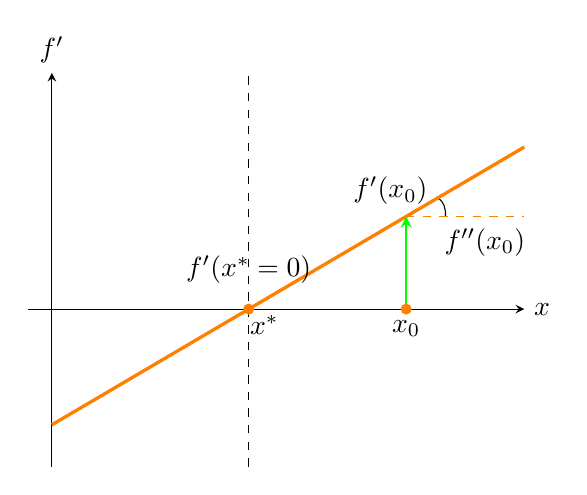
\begin{tikzpicture}[>=stealth]
        \draw[->](0,-2)--(0,3)node [above] {$f'$};
        \draw[->](-0.3,0)--(6,0)node[right]{$x$};
        \draw[dashed] (2.5,-2)--(2.5,3);
        \draw (5,1.176) to [out=90,in=330] (4.9,1.4112);
        \draw[very thick,draw=orange,domain=0:6] plot (\x,{0.588*\x-1.47});
        \fill[fill=orange] (2.5,0) circle[radius=0.07];
        \node at(2.7,-0.2) {$x^{*}$};
        \node at(2.5,0.5) {$f'(x^{*}=0)$};
        \draw[->,thick,draw=green] (4.5,0)--(4.5,1.176);
        \fill[fill=orange] (4.5,0) circle[radius=0.07];
        \node at(4.5,-0.25) {$x_{0}$};
        \draw[dashed,draw=orange] (4.5,1.176)--(6,1.176);
        \node at(4.3,1.5) {$f'(x_{0})$};
        \node at(5.5,0.85) {$f''(x_{0})$};
    \end{tikzpicture}
\end{center}
これによりニュートン法の最小化の近似値は
\begin{align*}
    x^{*}=x_{0}-\frac{1}{f''(x_{0})}f'(x_{0}) \tag{3.6}
\end{align*}
一般の場合のニュートン法では2次式を仮定して傾きを元に極値の位置を推定していく. しかし導関数によっては発散してしまう可能性がある.\\
多変数のニュートン法では以下のヘッセ行列(ヘシアン, ヘシアン行列)
となる.
\begin{align*}
    H(\mbox{\boldmath $x$}_{0})=\begin{pmatrix} \displaystyle \frac{\partial^{2}f(\mbox{\boldmath $x$}_{0})}{\partial x_{1}x_{1}}&\displaystyle  \frac{\partial^{2}f(\mbox{\boldmath $x$}_{0})}{\partial x_{1} \partial x_{2}} \\ \displaystyle \frac{\partial^{2}f(\mbox{\boldmath $x$}_{0})}{\partial x_{2} \partial x_{1}} &\displaystyle \frac{\partial^{2}f(\mbox{\boldmath $x$}_{0})}{\partial x_{2} \partial x_{2}} \end{pmatrix} 
\end{align*}
微小量の変化したときの変化量が0となればよいので
\begin{eqnarray*}
    \frac{\partial}{\partial \mbox{\boldmath $x$}}f(\mbox{\boldmath $x$}_{0}+\Delta \mbox{\boldmath $x$})&=&\nabla f(\mbox{\boldmath $x$}_{0})+H(\mbox{\boldmath $x$}_{0})\Delta \mbox{\boldmath $x$}=0\\
    \Delta \mbox{\boldmath $x$} &=& -H(\mbox{\boldmath $x$}_{0})^{-1}\nabla f(\mbox{\boldmath $x$}_{0})\\
    x^{*}&=&x_{0}-H(\mbox{\boldmath $x$}_{0})^{-1}\nabla f(\mbox{\boldmath $x$}_{0})\ \ (2次系の場合は即最適解)
\end{eqnarray*}
一般の場合は漸化式で
\begin{align*}
    x_{i+1}=x_{i}-H(\mbox{\boldmath $x$}_{i})^{-1}\nabla f(\mbox{\boldmath $x$}_{i})
\end{align*}
となる.\\\\
勾配法においては, 得られる解は初期値に依存する.